\documentclass{article}
\usepackage{tikz, comment}
\usepackage{pifont}
\usepackage{fontspec}
\usetikzlibrary{arrows, decorations.markings, decorations.pathreplacing}
\begin{comment}
:Title: Not defined yet
:Tags: revolution;length;figure;curve
:Author: Prof.Hu Ji-shan, HKUST
:Slug: No name yet

Description Here.........
\end{comment}
\begin{document}\centering

\newcommand{\AxisRotator}[1][rotate=0]{%
\tikz [x=0.25cm,y=0.60cm,line width=.2ex,-stealth,#1] \draw (0,0) arc (-165:165:1 and 1);%
}

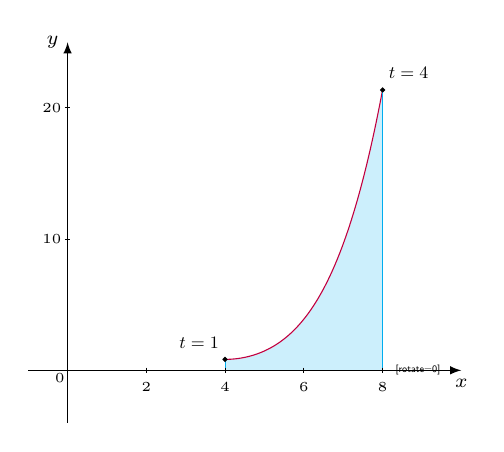
\begin{tikzpicture}[>=latex,xscale=.5*1, yscale=.5/3][font=\sf\small]

%\draw[xstep=1cm,ystep=1cm,color=gray!80] (0, -1) grid (8, 8);

\draw[white, fill=cyan!20] (4,0)--++(4, 0)--++(0,{(4)^3/3+1/(2*(4)^2)})--++(-4,0)--cycle;

\draw[white, fill=white, samples=100, smooth, domain=1:4, variable=\t]
plot ({4*sqrt(\t)}, {(\t)^3/3+1/(2*(\t)^2)})--({4}, {(4)^3/3+1/(2*(4)^2)});

\draw[purple, samples=100, smooth, domain=1:4, variable=\t]
plot ({4*sqrt(\t)}, {(\t)^3/3+1/(2*(\t)^2)});

\draw[cyan] (4,0)--++(0,{((1)^3/3+1/(2*(1)^2))});
\draw[cyan] (8,0)--++(0,{((4)^3/3+1/(2*(4)^2))});

\draw[fill, black, xscale=1/1, yscale=3] ({4*sqrt(1)*1}, {((1)^3/3+1/(2*(1)^2))/3}) circle(0.05)node[left, xshift=0, yshift=6, scale=0.7]{$t=1$};
\draw[fill, black, xscale=1/1, yscale=3] ({4*sqrt(4)*1}, {((4)^3/3+1/(2*(4)^2))/3}) circle(0.05)node[right, xshift=0, yshift=6, scale=0.7]{$t=4$};

\foreach \x in {2,4,6,8}
\draw (\x,2pt*3) -- (\x,-2pt*3)
node[anchor=north] {\tiny$\x$}
;

\foreach \x in {}
\draw (\x,2pt/2.5) -- (\x,-2pt/2.5)
node[anchor=south] {\tiny$\x$}
;
\foreach \y in {10, 20}
\draw (-2pt/1,\y) -- (2pt/1,\y)
node[anchor=east] {\tiny $\y$}
;

\draw[->] (-1, 0) -- (10, 0)node[below] {\scriptsize$x$} node [solid, midway, pos=0.9, scale=0.4]{\AxisRotator[rotate=0]};

\draw[-> ] (0, -4) -- (0, 25)node[left] {\scriptsize$y$} ;

\node[yshift=0] at (-0.2/1, -0.2*3) {\tiny$0$};

\end{tikzpicture}
\end{document}